%! TEX root = ../main.tex
% ==============================================================
% IMMUTABLE — generated automatically, do not edit this block
%
% — Provenance ───────────────────────────────────────────────────
%   script            : analysis_scratch/per40_full_chirp.py
%   computed_in       : analysis_scratch/per40_full_chirp.py (eta_{IN} overlay; raw + 25-sample rolling-mean smoothed; paddle-period grid anchored at first uc per condition)
%   plot_type         : per40_overlay
%   data_class        : DELEG
%   generated_at      : 2026-05-12T09:45:59
%   findings_doc      : memory/methodology_wind_enhances_A_in.md
%
% — Thesis context ──────────────────────────────────────────────
%   chapter           : 04
%   caption_label     : fig:ch04_per40_overlay_t40-51
%   caption_short     : Per40 nedstart, fase fortsatt skiftet
%
% — Filters ────────────────────────────────────────────────────
%   panel             : full
%   wind              : no, full
%   amplitude [V]     : 0.2
%   frequency [Hz]    : 1.3
%   probes            : 
%   run_category      : 
%   quality_flag      : ok
%   mooring           : 
%
% — Data provenance ────────────────────────────────────────────
%   n_runs            : 
%   in_probes_used    : 
%   out_probes_used   : 
%   probe_configs     : 
%   non_final_config_n: 
%   datasets        :
%     (none registered — set plot_utils.ACTIVE_DATASETS)
%   run_paths       :
%     (omitted — aggregate over > threshold runs, see datasets)
%
% — Method / numerical parameters ─────────────────────────────
%   grouper           : 
%   collapse_panels   : 
%   fft_window_hz     : 
%   extra_params      : zoom_window_s=(40, 51). label=ramp-down + decay. smoother=25 samples (100 ms). runs: nw=/Users/ole/Kodevik/wave_project/wavedata/20260327-ProbePos4_31_FPV_2-tett6roof-under9Mooring30-height100-lowrange/fullpanel-nowind-amp0200-freq1300-per40-depth580-mstop30-run1.csv, fw=/Users/ole/Kodevik/wave_project/wavedata/20260327-ProbePos4_31_FPV_2-tett6roof-under9Mooring30-height100-lowrange/fullpanel-fullwind-amp0200-freq1300-per40-depth580-mstop30-run1.csv.
%
% — Summary stats cited in caption ────────────────────────────
%   (none registered — pass extra_stats=... to build_fig_meta)
%
% — Subfigures available ───────────────────────────────────────
%     FIGURES/ch04_per40_overlay_t40-51.pdf
% ── end immutable block ─────────────────────────────────────────
\begin{figure}[htbp]
  \centering
  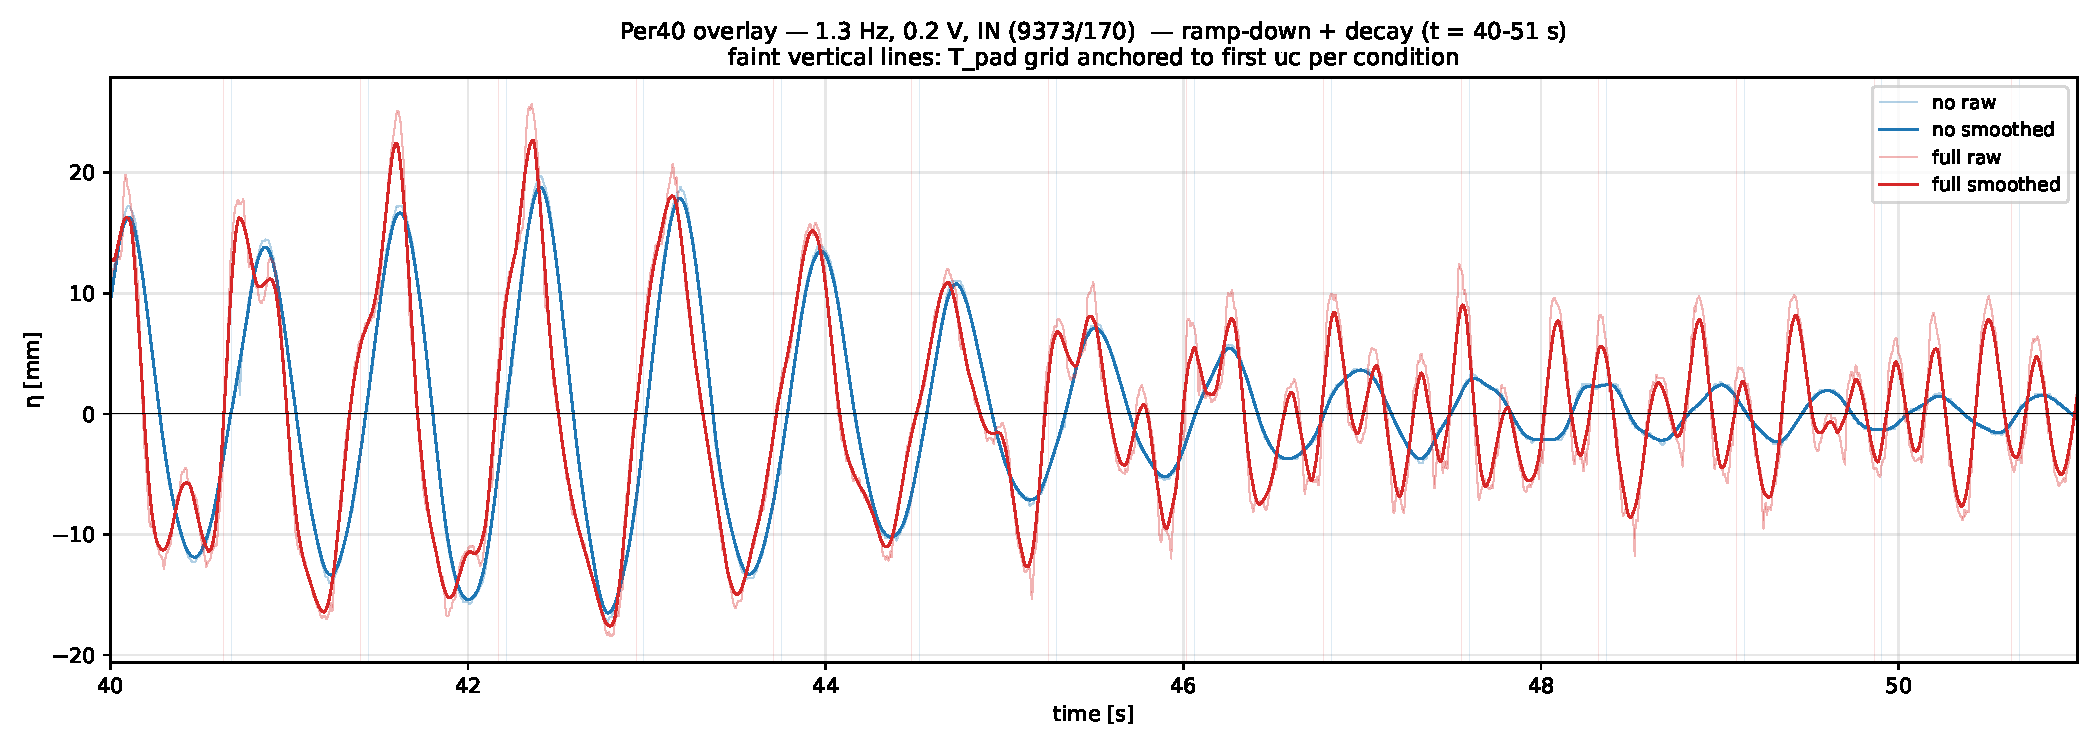
\includegraphics[width=\linewidth]{FIGURES/ch04_per40_overlay_t40-51.pdf}
% >>> CAPTION-SYNC START (do not edit this block; sync_captions.py overwrites)
  \caption{
    % TODO: write caption (edit FIGURE_CAPTIONS/TABLE_CAPTIONS)
  }
% <<< CAPTION-SYNC END
  \label{fig:ch04_per40_overlay_t40-51}
\end{figure}
